
We consider a multiphase flow with no-mass transfer, i.e. $\textbf{u}_k=\textbf{u}_I$.
The interfaces have negligible weight and no interfacial viscosity. 

\subsection{Mixture momentum equation and a constitutive expression for the bulk stress tensor}

As mentioned earlier in this manuscript we  now focus on the global suspension stress as this is a quantity of uppermost importance. 
Firstly, we expose the mixture or \textit{signle-fluid} formulation of the momentum equation following the procedure to derive \ref{eq:dt_f}.
It gives, 
\begin{equation}
    \pddt (\rho \textbf{u})
    \div (\rho \textbf{uu} - \bm{\sigma}^\text{eq})
    = \textbf{b}
    \label{eq:dt_avg_rho_u}
\end{equation}
where $\textbf{b}$ is a generic body force and the equivalent stress is defined as, 
\begin{equation}
    \bm{\sigma}^\text{eq}
    = - \avg{\textbf{u}'\textbf{u}'}
    + \avg{\chi_2\bm{\sigma}_2^0}
    + \avg{\chi_1\bm{\sigma}_1^0}
    + \avg{\delta_I \bm{\sigma}_I^0}. 
    \label{eq:sigma_eq_def}
\end{equation}
Under this form we can already state the trivial results which is that the equivalent stress of a medium is constituted by the averaged fluid stress, particles stress and the stress due to interfaces. 
As already noticed by \citet{batchelor1970stress} the surface stress presence in the suspension stress makes the mixture having characteristics of an elastic medium. 
Making the suspension going from a Newtonian fluid to a visco-elastic fluid. 

The expression \ref{eq:sigma_eq_def} is somewhat unpractical, indeed its makes appear the internal particle stress explicitly which we usually try to avoid in order to take apart the dispersed nature of the particle phase. 
Therefore, we msut seek for an expression of $\avg{\chi_1\bm{\sigma}_1^0}
+ \avg{\delta_I \bm{\sigma}_I^0}$ in terms of the particles Lagrangian properties seen in \ref{sec:Lagrangian}.
This will be done through the use of the momentum of momentum equations. 
From now on we will use indices notation to be more clear. 
The first step is to express these phase averaged fields into particle averaged fields. 
Actually, these stresses appear under the divergence operator in \ref{eq:dt_avg_rho_u}. 
Thus, following \ref{eq:f_exp} we express the divergence of the particle phase stress by, 
\begin{align}
    \label{eq:exp_sigma2}
    \partial_k \avg{\chi_2\bm{\sigma}_2^0}_{ik}
    &=  \partial_k\pOavg{ \bm{\sigma}^0_{2,ik}}
    - \partial_k\partial_j
    \pOavg{ r_j\bm{\sigma}^0_{2,ik}}        
    + \ldots  \\
    \label{eq:exp_sigmaI}
    \partial_k \avg{\delta_I \bm{\sigma}_I^0}_{ik} 
    &=  \partial_k\pSavg{ \bm{\sigma}_{I,ik} }
        - \partial_k\partial_j \pSavg{ r_j \bm{\sigma}_{I,ik} }
        + \ldots  
\end{align}
Notice that the second terms on the RHS of \ref{eq:exp_sigma2} and \ref{eq:exp_sigmaI} are subject to the double divergence operator $\partial_k\partial_j$. 
Therefore, only the symmetric part with respect to the index $k$ and $j$ will remain in this expression. 
Consequently, the particle phase averaged stress can be reformulated by, 
\begin{align}
    \label{eq:exp_sigma22}
    \partial_k \avg{\chi_2\bm{\sigma}_2^0}_{ik}
    &=  \partial_k\pOavg{ \bm{\sigma}^0_{2,ik}}
    -\frac{1}{2} \partial_k\partial_j
    \pOavg{ r_j \bm{\sigma}^0_{2,ik} + r_k\bm{\sigma}^0_{2,ij}}
    + \ldots  \\
    \label{eq:exp_sigmaI2}
    \partial_k \avg{\delta_I \bm{\sigma}_I^0}_{ik} 
    &=  \partial_k\pSavg{ \bm{\sigma}_{I,ik}^0 }
        -\frac{1}{2} \partial_k\partial_j \pSavg{ r_j \bm{\sigma}_{I,ik}^0+r_k \bm{\sigma}_{I,ij}^0 }
        + \ldots  
\end{align}
Such decomposition can be done at any order of accuracy, this has also been shown by \citet[Appendix A]{nott2011suspension} in a similar context. 
Now the challenge will be to replace the particle average of the zeroth and first order moment of the stress tensor. 
This is done by using the following expressions, 
\begin{align}
    \intS{ 
    (\bm{\sigma}_I)_{ik}
    }
    +\intO{ 
    (\bm{\sigma}_2^0)_{ik}
    }
    = 
    \intO{ \rho_2 
    (\textbf{w}_2^0\textbf{w}_2^0  )_{ik}
    }
    -\ddt \intO{ r_i (\textbf{u}^0_2)_k }
    +\intS{ 
        b_{i}
        r_k 
    }
    +\intS{ 
     r_i (\bm{\sigma}_1^0 \cdot \textbf{n}_2)_{k}
    }
    \label{eq:dt_P_alpha}\\
    \intO{ r_{j}(\bm{\sigma}^0_2)_{ki}+r_{k}(\bm{\sigma}^0_2)_{ji}}
    +\intS{ r_{j}(\bm{\sigma}^0_I)_{ki}+r_{k}(\bm{\sigma}_I^0)_{ji}}
    = 
    - \ddt\intO{ \rho_2 (\textbf{u}_2^0)_i r_j r_k }\nonumber\\
    + \intO{ \rho_2 (r_{j} (\textbf{w}_2^0)_k (\textbf{u}^0_2)_i + r_k (\textbf{w}_2^0)_j (\textbf{u}^0_2)_i)}
    +\intS{  r_{k}r_{j} (\bm{\sigma}_1^0)_{il} (\textbf{n}_2)_l }
    + \intO{ r_{k}r_{j}  \rho_2 b_i } 
    \label{eq:dt_P2_alpha}
\end{align}
which are the first and second order moments of momentum equations, respectively. 
The first order moment of momentum equation has been presented in \ref{sec:Lagrangian}. 
The second order moment expression has been derived using the generic formula, \ref{eq:dt_Q_n} with $n = 2$.
Additionally, in light of \ref{eq:dt_Q_n} any $n^\text{th}$ order terms in \ref{eq:exp_sigma22} and \ref{eq:exp_sigma22} can be substitued by the $n^\text{th}$ order moments of momentum equation. 
Remark that in a recent study of \citet{dolata2020heterogeneous} they derive an equivalent expression of \ref{eq:dt_P_alpha}  but with what they called energy method.  
Their, Equation (3.15) is in fact the equation of the moment of momentum to which we retrieve the RHS terms of \ref{eq:tau_1_final}, it is derived in the limit of stokes flows.




Substituting : the expression of $\avg{\chi_2\bm{\sigma}_2+ \delta_I\bm{\sigma}_I}$ using \ref{eq:exp_sigma22},\ref{eq:exp_sigmaI2}, \ref{eq:dt_P_alpha} and \ref{eq:dt_P2_alpha}, and the expression of $\avg{\chi_1\bm{\sigma}_1}$ using \ref{eq:sigma_eq1_def} one obtain the following expansion for the suspension stress,
\begin{multline*}
    \bm{\sigma}^\text{eq}
    = 
    - \rho_1 \avg{\chi_1\textbf{u}'_1\textbf{u}_1'}
    - m_p \pavg{\textbf{u}_\alpha'\textbf{u}_\alpha'}
    - m_p \textbf{u}_\alpha\textbf{u}_\alpha
    + \phi_2 \textbf{u}_2\textbf{u}_2
    % + \avg{\chi_1\bm{\sigma}_1^0}
    - \phi_1 p_1 \textbf{I}
    + \mu_1 \textbf{e}\\
    % + \avg{\chi_2\bm{\sigma}_2^0}
    % + \avg{\delta_I \bm{\sigma}_I^0}. 
    +\pSavg{r_i (\bm{\sigma}_1^0 \cdot \textbf{n}_2)_{k}}
    - \mu_1 \pSavg{(\textbf{u}_1 \textbf{n}_1)_{ik}+(\textbf{n}_1 \textbf{u}_1)_{ik}}
    % + \pOavg{ \rho_2 (\textbf{w}_2^0\textbf{w}_2^0  )_{ik}}
    -\pddt(n_p\mathcal{P}_{p,ik})
    +\pSavg{ b_{i}r_k }\\
    - \frac{1}{2}\partial_j\left[
        - \pddt (n_p\mathcal{P}_{p,ijk})
        % + \pOavg{ \rho_2 (r_{j} (\textbf{w}_2^0)_k (\textbf{u}^0_2)_i + r_k (\textbf{w}_2^0)_j (\textbf{u}^0_2)_i)} 
        + \mu_1 2\pSavg{(\textbf{r}\textbf{w}_2^0 \textbf{n}_1)_{jik}+(\textbf{r}\textbf{n}_1 \textbf{w}_2^0)_{jik}}
        \right.\\ \left.
        +\pSavg{ r_{k}r_{j} (\bm{\sigma}_1^0)_{il} (\textbf{n}_2)_l }
        + \pOavg{ r_{k}r_{j}  \rho_2 b_i } 
    \right]
    \label{eq:sigma_eq}
\end{multline*}
% \begin{multline*}
%     \bm{\sigma}^\text{eq}
%     = - \avg{\textbf{u}'\textbf{u'}}
%     % + \avg{\chi_1\bm{\sigma}_1^0}
%     - p_1 \textbf{I}
%     + \mu_1 \textbf{e}\\
%     % + \avg{\chi_2\bm{\sigma}_2^0}
%     % + \avg{\delta_I \bm{\sigma}_I^0}. 
%     - \mu_1 \pSavg{(\textbf{u}_1 \textbf{n}_1)_{ik}+(\textbf{n}_1 \textbf{u}_1)_{ik}}
%     + \pOavg{ \rho_2 (\textbf{w}_2^0\textbf{w}_2^0  )_{ik}}
%     -\pavg{\ddt \intO{ r_i (\textbf{u}^0_2)_k }}
%     +\pSavg{r_i (\bm{\sigma}_1' \cdot \textbf{n}_2)_{k}}
%     +\pSavg{ 
%         b_{i}
%         r_k 
%     }\\
%     - \frac{1}{2}\partial_j\left[
%         - \pavg{\ddt\intO{ \rho_2 (\textbf{u}_2^0)_i r_j r_k }}
%         + \pOavg{ \rho_2 (r_{j} (\textbf{w}_2^0)_k (\textbf{u}^0_2)_i + r_k (\textbf{w}_2^0)_j (\textbf{u}^0_2)_i)} \right.\\ \left.
%         + \mu_1 2\pSavg{(\textbf{r}\textbf{w}_2^0 \textbf{n}_1)_{jik}+(\textbf{r}\textbf{n}_1 \textbf{w}_2^0)_{jik}}
%         +\pSavg{ r_{k}r_{j} (\bm{\sigma}_1')_{il} (\textbf{n}_2)_l }
%         + \pOavg{ r_{k}r_{j}  \rho_2 b_i } 
%     \right]
%     \label{eq:sigma_eq}
% \end{multline*}
Notice that according the discussion in the previous section we could add and subtracted $\phi_2 p_1$ to remove the volume fraction factor in front of $p_1$.
Let's compare this expression to the one obtained by \citet{zhang1997momentum}. 
Firstly, notice that we recovered the moments of the surface traction term plus the contribution to the surface velocity integral coming from \ref{eq:tau_1_final}. 
In \citet{zhang1997momentum} the surface traction terms are grouped under the terms $\bm{\Sigma}_1$ and $\bm{\Sigma}_2$.
In our formulation we did not retrieve the mean contribution from the stress $\bm{\sigma}_1$ to the exchange terms nevertheless it can be recovered easily yielding an equivalent expression for the moments of the surface traction. 
The surface velocity contribution terms also grouped in $\bm{\Sigma}_1$ and $\bm{\Sigma}_2$ might seem different from the ones derived here. 
This is due to the facts that in \citet{zhang1997momentum} the surface velocity contribution terms are derived from \citet{eq:tau_1} where we used \ref{eq:tau_1_final}, it is nevertheless equivalent. 
Where our expression might differ from \citet{zhang1997momentum} is regarding what they called the acceleration term $\bm{\Sigma}_a$ in fact contains all the terms on the RHS of the expression \ref{eq:dt_P_alpha}.
In our formulation however, we included the second order moment of the particles' acceleration, i.e. the RHS of \ref{eq:dt_P2_alpha}.
But above all, we reformulated the dispersed phase Reynolds stress tensor $\avg{\chi_2\rho_2 \textbf{u}_2 \textbf{u}_2}$ to show that it in fact canceled some moments of the terms on the RHS of \ref{eq:dt_P_alpha} and \ref{eq:dt_P2_alpha} letting us only with the partial derivative of the moments of momentum of arbitrary order.
The consequence of this is the apparition of the particle Reynolds stress $\pavg{\textbf{u}_\alpha'\textbf{u}_\alpha'}$. 
This last manipulation is in fact obvious when one consider \ref{eq:scheme_equivalence}, and is the reason why our $\bm{\Sigma}_R$ and $\bm{\Sigma}_a$.

We believe that under the form of \ref{eq:sigma_eq} the contribution of the particle to the suspension stress is more physical. 
Indeed, it consists into three distinct contribution. 
The first one is the contribution from the surface traction moments in which we include the surface velocity terms in light of \ref{eq:stresslet_def}. 
The second contribution comes from the partial time derivative of the first moments. 
Which we recall represent the acceleration of the first and higher order kinematic of the particles such as angular acceleration, stretching etc\ldots
And the last contribution coming from the body forces and higher moments of the body force. 
Notice that on the RHS of \ref{eq:dt_avg_rho_u} we have the continuous averaged body force term, which might be expressed as, 
$
    \textbf{b}
    = \phi_1 \textbf{b}_1 
    + \pOavg{\textbf{b}}
    - \div \pOavg{\textbf{r} \textbf{b}}
    \ldots
$
and so on. 
This implies that the moments of the body force play no dynamical role in \ref{eq:sigma_eq} as the same moments appear twice with opposite sign. 
This is in agreement with \citet{dolata2020heterogeneous} which reached the same conclusion, limited to stoke flows, however. 
The only difference wit stokes flow is that in our case the skew part of the stress might come form the angular acceleration of the particles. 

In \citet{dolata2020heterogeneous} they stipulate that the surface tension effect plays no role in the suspension Rheology. 
This is indeed what we found as witnessed by the absence of surface tension terms in \ref{eq:sigma_eq} however it must be understood that surface tension force will play a role in the evolution equation of the different moment of momentum which appear in \ref{eq:sigma_eq}. 
Thus, the statement of \citet{dolata2020heterogeneous} might be reformulated as the surface tension effect plays no explicit role in the suspension Rheology. 

The skew-symmetric part of the stress can come form severals contribution. 
The moment of momentum that can be skew-symmetric if the particles posses angular acceleration. 
The moments of the body forces, which can also yields skew-symmetric components. 
And obviously, the torque 

In a recent study \citet{wolgemuth2023continuum} found out that the bulk stress of a stokestain suspension of spherical particles contained an antisymmetric tensor responsible for self torquing. 
We believe that such stress is found to be, in our formulation related to the terms, $\pOavg{r_{k}r_{j}  \rho_2 b_i }$ which in the case of solid spherical particle can be expressed as $n_p\mathcal{I}_p \textbf{b}_p$ which appear under the divergence operator. 
In \citet{wolgemuth2023continuum} they obtain the term \ldots
However, it can be shown that such stress is not present in \ref{eq:dt_avg_rho_u}. 
\tb{citer jackson}
\tb{Comparer avec Zhang 1997 it seem similar }

\tb{Additionally, th e cancellation of the higher moments isn't trivial therefore it might be considered to show that no anti symmetric part exist except the torque}

\tb{dire que wolgemouth s'est trompe}

\tb{Faire le lien avec la mixture equaiton de jackson et peut etre de zhang ?}

where the derivative of the surface plays the role of an elastic bahavior \citet[appendix A]{batchelor1970stress}.

Now, let discus the antisymmetric part of the stress tensor. 
As, it is done in \cite{dolata2020heterogeneous} we start our demonstration from the local angular acceleration principle inside the particle phase, namely \cite[chapter 2]{leal2007advanced},
\begin{equation}
    \epsilon_{ijk} : \bm{\sigma}_{2,kj}^0 = 0 
\end{equation}
which holds as long as no body torque are present.
It is assumed true here.  
Upon taking the appropriate average we obtain the averaged angular momentum equation : 
\begin{equation*}
    \epsilon_{ijk} : \avg{\chi_2 \bm{\sigma}_2^0}_{kj} = 0 
\end{equation*}
Expanding the averaged stress about the particles center yields the expression,
\begin{align}
    \label{eq:exp_sigma2}
     \epsilon_{ijk}\avg{\chi_2\bm{\sigma}_2^0}_{kj}
    &=  \epsilon_{ijk}\pOavg{ \bm{\sigma}_2^0}_{kj}
    - \epsilon_{ijk}\partial_l
    \pOavg{ r_l(\bm{\sigma}_2^0)_{kj}}        
    + \ldots  \\
    &=  \epsilon_{ijk}\pOavg{ \bm{\sigma}_2^0}_{kj}
    - \epsilon_{ijk}\partial_l\bm{\Sigma}_{kj}\\
    % \label{eq:exp_sigmaI}
    %  \avg{\delta_I \bm{\sigma}_I^0}_{ik} 
    % &=  \pSavg{ (\bm{\sigma}_I)_{ik} }
    %     - \partial_j \pSavg{ r_j (\bm{\sigma}_I)_{ik} }
    %     + \ldots  
\end{align}
where $\bm{\Sigma}$ contain all the higher order terms. 
Now, by Substituting the expression of $\pOavg{\sigma_{2,kj}^0}$ with the first moment of momentum equaiton one can show that, 
\begin{equation*}
    \ddt \mu_i +  \epsilon_{ijk} \pOavg{b_k r_j}
    + \pSavg{r_i \sigma_{1,k}^0n_{2,k}}
    - \epsilon_{ijk}\partial_l\bm{\Sigma}_{kj} = 0 
\end{equation*}
where we recall that $\mu_i$ is the angular momentum. 
It is now evident that if no angular momentum, nor moment of body force, nor torque exist we obtain : $\div \bm{\Sigma} = 0$.
This indicates that the antisymmetric part of the averaged particle stress exist only in the presence of one of the terms cite above. 

However, these conditions might be relaxed since, as we observed earlier  neither the moments of the body forces nor the moments of momentum, played a dynamical role in the momentum averaged equation. 
Which let us with the hydrodynamic torque as the only remaining first order term in the stress.
Therefore, the equivalent stress of a suspension is symmetric unless a couple is exerted by the carrier fluid on the particles. 


\subsubsection{Second decomposition of the flux term}
In the same spirit as \citet{chu2016flux} we wish to make appear the ensemble averaged bulk stress into the continuous and dispersed phase equations instead of the fluid averaged bulk stress. 
Thus, for the dispersed phase eq, we first use the expression :
\begin{align*}
    \div  (\phi_1 \mathbf{\Phi}_1)
    + \avg{\delta_I \mathbf{\Phi}_1^0 \cdot \textbf{n}_1}
    &=
    \div  (\phi_1 \mathbf{\Phi}_1)
    + \avg{\delta_I \mathbf{\Phi}_1' \cdot \textbf{n}_1}
    + \mathbf{\Phi} \cdot  \avg{\delta_I \textbf{n}_1}\\
    &=
    \div  (\phi_1 \mathbf{\Phi}_1)
    + \avg{\delta_I \mathbf{\Phi}_1' \cdot \textbf{n}_1}
    - \mathbf{\Phi} \cdot  \avg{\grad\chi_1}\\
    &=
    \div  \avg{\chi_1 \mathbf{\Phi}_1'}
    + \avg{\delta_I \mathbf{\Phi}_1' \cdot \textbf{n}_1}
    + \phi_1 \div \bm{\Phi}\\
\end{align*}
If we introduce the decomposition  $\mathbf{\Phi}_1^0 =  \mathbf{\Phi} + \mathbf{\Phi}_1'$.
Thus, $\avg{\chi_1\mathbf{\Phi}_1'} 
= \avg{\chi_1 \mathbf{\Phi}_1^0} - \avg{\chi_1\mathbf{\Phi}}
= \phi_1 (\mathbf{\Phi}_1 - \mathbf{\Phi})
= \phi_1 ( \phi_2 (\mathbf{\Phi}_1  -  \mathbf{\Phi}_2)  - \phi_I \mathbf{\Phi}_I )$
\subsection{Chu et al derivation is not good}
We first have $\bm{\Phi} = \phi_2 \bm{\Phi}_2+\phi_1 \bm{\Phi}_1 + \phi_I \bm{\Phi}_I$. 
Besides,
\begin{align*}
    \div  (\phi_1 \mathbf{\Phi}_1)
    - \avg{\delta_I \mathbf{\Phi}_1^0 \cdot \textbf{n}_2}
    &=
    \div  \mathbf{\Phi}
    - \div  (\phi_2\mathbf{\Phi}_2)
    - \div  (\phi_I\mathbf{\Phi}_I)
    - \avg{\delta_I \mathbf{\Phi}_1^0 \cdot \textbf{n}_2}\\
    &=
    \div  \mathbf{\Phi}
    + \avg{ [(\mathbf{\Phi}_2^0 - \mathbf{\Phi}_1^0) \cdot \textbf{n}_2 - \div \mathbf{\Phi}_I^0]\delta_I}
    - \avg{ \chi_2 \div \mathbf{\Phi}_2^0  }\\
    &- \avg{ \mathbf{\Phi}_I^0  \cdot \grad\delta_I}
    \\
    &=
    \div  \mathbf{\Phi}
    - \avg{ \chi_2 \div \mathbf{\Phi}_2^0  }
    - \avg{ \mathbf{\Phi}_I^0  \cdot \grad\delta_I}
    \\
    &=
    \phi_1 \div  \mathbf{\Phi}
    - \avg{ \chi_2 \div \mathbf{\Phi}_2'  }
    - \avg{ \mathbf{\Phi}_I^0  \cdot \grad\delta_I}
    \\
\end{align*}
Where we have assume a jump conditioon of the form $\sum_k \Jump{\mathbf{\Phi}_k^0} = \div \bm{\Phi}_I^0$ and the definition $\bm{\Phi}'_2 = \bm{\Phi}_2^0 - \bm{\Phi}$.


The second term can be reformulated as a series expansion such that 
$\avg{ \chi_2 \div \mathbf{\Phi}_2^0  } = \pavg{\int_{\Omega_\alpha} \div \mathbf{\Phi}_2^0 d\Omega} - \div\pavg{\int_{\Omega_\alpha} \textbf{r} \div \mathbf{\Phi}_2^0 d\Omega} \ldots $
Upon using the divergence theorem on these terms we obtain :
\begin{align*}
    \div  (\phi_1 \mathbf{\Phi}_1)
    - \avg{\delta_I \mathbf{\Phi}_1^0 \cdot \textbf{n}_2}
    &=
    \div  \mathbf{\Phi}
    - \avg{ \mathbf{\Phi}_I^0  \cdot \textbf{n}\cdot\grad(\textbf{n} \delta_I)}\\
    &- \pavg{\int_{\Omega_\Sigma} \textbf{n}_2 \cdot \mathbf{\Phi}_2^0 d\Sigma} 
    + \div\pavg{\int_{\Sigma_\alpha}  \textbf{n}_2 \cdot \textbf{r}\mathbf{\Phi}_2^0 d\Sigma} 
    + \div\pavg{\int_{\Omega_\alpha}  \mathbf{\Phi}_2^0 d\Omega} \ldots
    \\
\end{align*}
Again we assumed a relation of the form $\sum_k \Jump{\mathbf{\Phi}_k^0} = \div \bm{\Phi}_I^0$. 

\subsection{Momentum $2^\text{nd}$ decomposition}
In this formulation the stress of reference is $\bm{\sigma}$.
Thus, the momentum equaiton takes the form,
\begin{align*}
    \pddt (\rho_1\phi_1 \textbf{u}_1 )
    + \div (\rho_1\phi_1 \textbf{u}_1  \textbf{u}_1
    + \bm{\sigma}^\text{eff}_1 )
    &= 
    \phi_1( \textbf{b}_1  +\div  \bm{\sigma})
    - n_p\textbf{F}_p \\
    % \pddt (\phi_2  \rho_2\textbf{u}_2)
    % + \div (
    %     \rho_2\phi_2 \textbf{u}_2\textbf{u}_2
    %     + \bm{\sigma}^\text{eff}_2
    %     )
    % &= 
    %  \phi_2 (
    %   \textbf{b}_2
    % + \div \bm{\sigma}_1 )
    % + n_p\textbf{F}_p ,
\end{align*}
With the following definition, 
\begin{align*}
    \bm{\sigma}^\text{eff}_1
    &=\rho_1 \phi_1 \oneavg{\textbf{u}_1'\textbf{u}_1'}
    - \phi_1 \oneavg{\bm{\sigma}_1'}
    - n_p\textbf{M}_p 
    \\
    \bm{\sigma}^\text{eff}_2
    &= \rho_2\phi_2 \twoavg{ \textbf{u}_2'\textbf{u}_2'} 
    + n_p\textbf{M}_p 
    +\bm{\sigma}_1 - \bm{\sigma},
\end{align*}
What is the form of 
$\phi_1 \oneavg{\bm{\sigma}_1'}
 = \avg{\chi_1 \bm{\sigma}_1^0}
 - \phi_1\bm{\sigma}
$. 
By considering $\bm{\sigma}_k^0 = -p_k^0 \textbf{I} + \mu_k \textbf{e}_k^0$
\begin{align*}
    \phi_1 \oneavg{\bm{\sigma}_1'}
 &= \avg{\chi_1 (-p_1^0 \textbf{I} + \mu_1 \textbf{e}_1^0)}
 - \phi_1\avg{-p^0 \textbf{I} + \mu \textbf{e}^0}\\
 &=  - \phi_1 p_1 \textbf{I} + \phi_1 \mu_1 \textbf{e}_1
 + \phi_1 p \textbf{I} + \phi_1 \avg{\mu^0 \textbf{e}^0}\\
 &=  - \phi_1 (p_1 - p) \textbf{I} 
 + \phi_1 \mu_1 \textbf{e}_1 
 - \phi_1 \avg{\mu^0 \textbf{e}^0}
\end{align*}
The last term is actually, 

Also, 
\begin{align*}
    \bm{\sigma}
    &= -\avg{\sum_k \chi_k p_k} I + \sum_k\mu_k \avg{\chi_k  (\grad\textbf{u}_k^0+(\grad\textbf{u}_k^0)^T)}\\
    &= -\avg{\sum_k \chi_k p_k} I + \sum_k\mu_k [\grad (\phi_k\textbf{u}_k)+ \grad (\phi_k\textbf{u}_k)^T
    + \avg{(\textbf{u}_k^0  \textbf{n}_k +  \textbf{n}_k\textbf{u}_k^0)\delta_I}]
\end{align*}

\subsubsection{Accurate description of the dispersed phase}


By adding \ref{eq:avg_dt_chi_f} and \ref{eq:avg_dt_delta_f} we obtain 
\begin{align*}
    \pddt \avg{\chi_2 f_2^0 +\delta_If_I^0}
    &= \div \avg{\chi_2 \mathbf{\Phi}_2^0 + \delta_I \mathbf{\Phi}_{I||}^0 - \chi_2 f_2^0 \textbf{u}_2^0 - \delta_I f_I^0 \textbf{u}_I^0}
    + \avg{\chi_2 \textbf{S}_2^0 }\\
    &+ \avg{\delta_I\textbf{S}_I^0} 
    + \avg{\delta_I\left[
        \mathbf{\Phi}_1^0
        + f_1^0
        \left(
            \textbf{u}_I^0
            - \textbf{u}_1^0
        \right)
    \right]
    \cdot \textbf{n}_2},
\end{align*}
To be consistent with \ref{eq:hybrid_avg_dt_chif} we must add and substract $\oneavg{\mathbf{\Phi}}\cdot\grad \avg{\chi_1} = \div  (\phi_1 \oneavg{\mathbf{\Phi}}) - \phi_1 \div \oneavg{\mathbf{\Phi}}$ the remaining terms must be added to the stress which gives,
\begin{align*}
    \div \avg{\chi_2 \mathbf{\Phi}_2^0 + \delta_I \mathbf{\Phi}_{I||}^0}
    & + \avg{\delta_I \bm{\Phi}_1 \cdot \textbf{n}_2}
    =
    \div \avg{\chi_2 \mathbf{\Phi}_2^0 + \delta_I \mathbf{\Phi}_{I||}^0}
    + \div \avg{\bm{\Phi}_1 \chi_1} 
     - \phi_1 \div \bm{\Phi}_1\\
    &= \div \bm{\Phi}
     - \phi_1 \div \bm{\Phi}_1
     =  \div (\bm{\Phi} - \bm{\Phi}_1)
     + \phi_2 \div \bm{\Phi}_1\\
\end{align*}
Under this form the dispersed phase equation reads, 
\begin{multline*}
    \pddt (\phi_2 f_2 +a_If_I)
    + \div (
        \phi_2 f_2 \textbf{u}_2
        + \phi_I f_I \textbf{u}_I
        + \phi_2 \twoavg{f_2'\textbf{u}_2'} 
        + \phi_I \Iavg{f_I'\textbf{u}_I'}
        + n_p \textbf{M}_p 
        )\\
    = 
    \div (\mathbf{\Phi}  - \mathbf{\Phi}_1 )
    + \phi_2 \div \mathbf{\Phi}_1 
    + \phi_2 \textbf{S}_2
    + \phi_I \textbf{S}_I
    + n_p\textbf{F}_p
\end{multline*}
It must be noted that $\mathbf{\Phi}  - \mathbf{\Phi}_1 
= \phi_I\mathbf{\Phi}_I+\phi_2(\mathbf{\Phi}_2  - \mathbf{\Phi}_1) $

If we try with the second form we must subtract and add $\avg{\delta_I \bm{\Phi} \cdot \textbf{n}_2}$, 
\begin{align*}
    \div \avg{\chi_2 \mathbf{\Phi}_2^0 + \delta_I \mathbf{\Phi}_{I||}^0}
    & + \avg{\delta_I \bm{\Phi} \cdot \textbf{n}_2}
    =
    \div \avg{\chi_2 \mathbf{\Phi}_2^0 + \delta_I \mathbf{\Phi}_{I||}^0 + \bm{\Phi} \chi_1} 
     - \phi_1 \div \bm{\Phi}\\
    &=
    \div \avg{\chi_2 \mathbf{\Phi}_2^0 + \delta_I \mathbf{\Phi}_{I||}^0 - \bm{\Phi} \chi_2} 
     + \phi_2 \div \bm{\Phi}\\
    &=
    \div \left(\phi_2 \mathbf{\Phi}_2 + \phi_I \mathbf{\Phi}_{I||} - (\bm{\Phi}_1 \phi_1 + \bm{\Phi}_2 \phi_2  + \bm{\Phi}_I \phi_I   ) \phi_2 \right) 
     + \phi_2 \div \bm{\Phi}\\
    &=
    \div \left(\phi_2 \mathbf{\Phi}_2 \phi_1 + \phi_I \mathbf{\Phi}_{I||} \phi_1 - \bm{\Phi}_1 \phi_1 \phi_2 \right) 
     + \phi_2 \div \bm{\Phi}\\
    &=
    \div \left(\phi_1 \mathbf{\Phi} - \bm{\Phi}_1 \phi_1 \right) 
     + \phi_2 \div \bm{\Phi}\\
\end{align*}


\subsection{Momentum equation}
The momentum equation of the continuous and dispersed phase now reads as, 
\begin{align*}
    \pddt (\rho_1\phi_1 \textbf{u}_1 )
    + \div (\rho_1\phi_1 \textbf{u}_1  \textbf{u}_1
    + \bm{\sigma}^\text{eff}_1 )
    &= 
    \phi_1( \textbf{b}_1  +\div  \bm{\sigma}_1)
    - n_p\textbf{F}_p \\
    \pddt (\phi_2  \rho_2\textbf{u}_2)
    + \div (
        \rho_2\phi_2 \textbf{u}_2\textbf{u}_2
        + \bm{\sigma}^\text{eff}_2
        )
    &= 
     \phi_2 (
      \textbf{b}_2
    + \div \bm{\sigma}_1 )
    + n_p\textbf{F}_p ,
\end{align*}
With the following definition, 
\begin{align*}
    \bm{\sigma}^\text{eff}_1
    &=\rho_1 \phi_1 \oneavg{\textbf{u}_1'\textbf{u}_1'}
    - n_p\textbf{M}_p 
    + \frac{1}{2}\grad (n_p \textbf{M}_p^2)
    \\
    \bm{\sigma}^\text{eff}_2
    &= \rho_2\phi_2 \twoavg{ \textbf{u}_2'\textbf{u}_2'} 
    + n_p\textbf{M}_p 
    - \frac{1}{2}\grad (n_p \textbf{M}_p^2)
    +\bm{\sigma}_1 - \bm{\sigma},
\end{align*}
\todo{\citep{prosperetti2004average} included teh higher moment of traction}
Note that  $\bm{\sigma}_1 - \bm{\sigma} =  \phi_2 (\bm{\sigma}_1  - \bm{\sigma}_2) - \phi_I \bm{\sigma}_I$
In these equations it is evident that the important closure is in $\sigma_1$ and $\sigma_2$.
\todo[inline]{In this section the local quantity are defined with the superscript $^0$}
The single-fluid formulation of the averaged momentum equation is obtained adding the two previous equation and reads,
\begin{equation}
    \pddt (\rho u_i)
    + \partial_k \cdot (\rho u_i u_k - \sigma_{ik}^\text{eff})
    = b_i. 
    \label{eq:dt_rho_u}
\end{equation}
Where $\textbf{u}$,$\bm{\sigma}^\text{eff}$ and \textbf{b} are the averaged velocity, stress tensor and body force, respectively. 
Thus, the bulk stress of a mixture can be written : 
\begin{equation}
    \sigma_{ik}^\text{eff}
    = \avg{\bm{\sigma}^0}_{ik}
    + \avg{\textbf{u}'\textbf{u}'}_{ik}
    = \avg{\chi_1 \bm{\sigma}^0_1}_{ik} 
    - \avg{\textbf{u}'\textbf{u}'}_{ik}
    +\avg{\chi_2 \bm{\sigma}^0_2}_{ik}
    + \avg{\delta_I \bm{\sigma}_I}_{ik}
    \label{eq:sigma}
\end{equation}
where $\bm{\sigma}_1$,$\bm{\sigma}_1$ and $\bm{\sigma}_I$  is the stress of the continuous phases, dispersed phase and on the interface, respectively.

\subsection{The fluid stress or averaged strain rate}
Regarding the fluid stress it can be reformulated considering Newtonian fluid,
\begin{equation}
    \phi_1 \bm{\sigma}_1 
    = - \phi_1 p_1 \textbf{I}
    + \mu_1 \phi_1 \textbf{e}_1
\end{equation}
with $\textbf{e}_1$ being the averaged shear rate. 
The first model is then, 
\begin{align*}
    \phi_1 \textbf{e}_1
    &= \avg{\chi_1 (\grad \textbf{u}_1^0+(\grad \textbf{u}_1^0)^T)}\\
    &= \grad (\phi_1\textbf{u}_1)+ \grad (\phi_1\textbf{u}_1)^T
    + \avg{(\textbf{u}_1^0  \textbf{n}_1 +  \textbf{n}_1\textbf{u}_1^0)\delta_I}\\
    &= \phi_1 (\grad \textbf{u}_1+ (\grad \textbf{u}_1)^T)
    + \avg{[(\textbf{u}_1^0 - \textbf{u}_1)  \textbf{n}_1 +  \textbf{n}_1(\textbf{u}_1^0 - \textbf{u}_1 )]\delta_I}\\
    &= \phi_1 (\grad \textbf{u}_1+ (\grad \textbf{u}_1)^T)
    + \avg{(\textbf{u}_1' \textbf{n}_1 +  \textbf{n}_1\textbf{u}_1')\delta_I}\\
\end{align*}
In \citet[chap 9]{ishii2010thermo} they assume,
\begin{equation}
    \avg{[(\textbf{u}_1^0 - \textbf{u}_1)  \textbf{n}_1 +  \textbf{n}_1(\textbf{u}_1^0 - \textbf{u}_1 )]\delta_I}\\
    = 
    (\textbf{u}_2 - \textbf{u}_1)  \grad \phi_1 +  \grad \phi_1(\textbf{u}_2 - \textbf{u}_1 )\\
\end{equation}
In our case 
\begin{equation}
    \sym{\avg{(\textbf{u}_1^0 - \textbf{u}_1)  \textbf{n}_1\delta_I } }\\
    = 
    \sym{\avg{\textbf{u}_1^0  \textbf{n}_1\delta_I  } }\\
    - \sym{\textbf{u}_1 \grad \phi_1 }\\
\end{equation}
the first term can be written, 
\begin{align}
    \avg{\textbf{u}_1^0  \textbf{n}_1\delta_I  }
    &=
    \pavg{\int_{\Sigma_\alpha} \textbf{u}_1^0  \textbf{n}_1 d\Sigma  }
    -\div \pavg{\int_{\Sigma_\alpha} \textbf{r}\textbf{u}_1^0  \textbf{n}_1 d\Sigma  }\\
    &=
    - \pavg{\int_{\Omega\alpha} \grad \textbf{u}_2^0   d\Omega   }
    + \div \pavg{\int_{\Omega\alpha} \grad (\textbf{ru}_2^0 )  d\Omega   }\\
    &=
    - \pavg{\int_{\Omega\alpha} \grad \textbf{u}_2^0   d\Omega   }
    + \div\pavg{\int_{\Omega\alpha} \textbf{u}_2^0   d\Omega   }
    + \div\pavg{\int_{\Omega\alpha} \textbf{r} \grad (\textbf{u}_2^0 )  d\Omega   }
\end{align}
where we used the velocity continuity at the interface. 

So it is a mean contribution minus the particles scale dissipation. 
The last term can actually be evaluated using the moment of momentum equation. 
In fact, it is better to write, 
Also,
\begin{align}
    \avg{(\textbf{u}_1^0 \textbf{n}_1 +  \textbf{n}_1\textbf{u}_1^0)\delta_I}
    = \avg{\grad(\textbf{u}_2^0 \chi_2) +  \grad(\chi_2\textbf{u}_2^0)^T}
    - \avg{\chi_2 (\grad\textbf{u}_2^0 + \grad(\textbf{u}_2^0 )^T)}
\end{align}
thus,
\begin{align*}
    \phi_1 \textbf{e}_1
    = \grad \textbf{u}+ (\grad \textbf{u})^T
    - \avg{\chi_2 (\grad\textbf{u}_2^0 + \grad(\textbf{u}_2^0 )^T)}
    = \textbf{e}
    - \phi_2 \textbf{e}_2
\end{align*}




Therefore, 
\begin{align*}
    \phi_1 \bm{\sigma}_1 
    &= - \phi_1 p_1 \textbf{I}
    + \mu_1 \textbf{e}
    - \lambda \avg{\mu_2 \chi_2 \textbf{e}^0_2}\\
    &= - \phi_1 p_1 \textbf{I}
    + \mu_1 \textbf{e}
    - \lambda \phi_2 \bm{\sigma}_2
    - \lambda \phi_2 p_2 \textbf{I}\\
    &= - (\phi_1 p_1+ \lambda \phi_2 p_2) \textbf{I}
    + \mu_1 \textbf{e}
    - \lambda \phi_2 \bm{\sigma}_2\\
\end{align*}
with $\textbf{e} = [\grad \textbf{u}+ (\grad \textbf{u})^T]$ and 
and $\lambda \mu_2 = \mu_1$.
Alternatively  this can be written, 
\begin{align*}
    \bm{\sigma}_1 
    &= - \left(p_1 + \frac{\lambda \phi_2}{\phi_1} p_2\right) \textbf{I}
    + \frac{\mu_1}{\phi_1} \textbf{e}
    - \frac{\lambda \phi_2}{\phi_1} \bm{\sigma}_2
\end{align*}
Now let's focus on the stress acting on the continuous phase, 
\begin{align*}
    \bm{\sigma}_1 - \bm{\sigma}
    &= \phi_2 \bm{\sigma}_1  
    - \phi_2\bm{\sigma}_2 - \phi_I \bm{\sigma}_I\\
    &=- \phi_2 \left(p_1 + \frac{\lambda \phi_2}{\phi_1} p_2\right) \textbf{I}
    + \frac{\mu_1\phi_2}{\phi_1} \textbf{e}
    - \frac{\lambda \phi_2^2}{\phi_1} \bm{\sigma}_2
    - \phi_2\bm{\sigma}_2 - \phi_I \bm{\sigma}_I\\
    &=- \phi_2 \left(p_1 + \frac{\lambda \phi_2}{\phi_1} p_2\right) \textbf{I}
    + \frac{\mu_1\phi_2}{\phi_1} \textbf{e}
    - \phi_2\bm{\sigma}_2 \left(
        \frac{\lambda \phi_2}{\phi_1} + 1
    \right)
    - \phi_I \bm{\sigma}_I\\
\end{align*}
Finally the bulk stress expression, 
\begin{align*}
    \bm{\sigma}
    &= \phi_1 \bm{\sigma}_1 
    +\phi_2 \bm{\sigma}_2 
    +\phi_I \bm{\sigma}_I \\
    &= - (\phi_1 p_1 + \lambda \phi_2 p_2) \textbf{I}
    + \mu_1 \textbf{e}
    + \bm{\sigma}_2 \phi_2 (1 - \lambda)
    +\phi_I \bm{\sigma}_I \\
\end{align*}

$
= \phi_1 (\mathbf{\Phi}_1 - \mathbf{\Phi})
= \phi_1 ( \phi_2 (\mathbf{\Phi}_1  -  \mathbf{\Phi}_2)  - \phi_I \mathbf{\Phi}_I )$


To summary we have, 
\begin{align*}
    \bm{\sigma}_1 
    &= - \left(p_1 + \frac{\lambda \phi_2}{\phi_1} p_2\right) \textbf{I}
    + \frac{\mu_1}{\phi_1} \textbf{e}
    - \frac{\lambda \phi_2}{\phi_1} \bm{\sigma}_2 \\
    \bm{\sigma}
    &= - (\phi_1 p_1 + \lambda \phi_2 p_2) \textbf{I}
    + \mu_1 \textbf{e}
    + \bm{\sigma}_2 \phi_2 (1 - \lambda)
    +\phi_I \bm{\sigma}_I \\
    \bm{\sigma}_1 - \bm{\sigma}
    &=- \phi_2 \left(p_1 + \frac{\lambda \phi_2}{\phi_1} p_2\right) \textbf{I}
    + \frac{\mu_1\phi_2}{\phi_1} \textbf{e}
    - \phi_2\bm{\sigma}_2 \left(
        \frac{\lambda \phi_2}{\phi_1} + 1
    \right)
    - \phi_I \bm{\sigma}_I\\
\end{align*}

\subsubsection{The solid particle case ($\lambda = 0$)}
In this case $\lambda = 0$ therefore, 
In agreement with \citet{jackson1997locally} and \citet{zhang1997momentum}. 
\begin{align*}
    \bm{\sigma}_1 
    &= - p_1  \textbf{I}
    + \frac{\mu_1}{\phi_1} \textbf{e}\\
    \bm{\sigma}
    &= - \phi_1 p_1 \textbf{I}
    + \mu_1 \textbf{e}
    + \bm{\sigma}_2 \phi_2 
    +\phi_I \bm{\sigma}_I \\
    \bm{\sigma}_1 - \bm{\sigma}
    &=- \phi_2 p_1  \textbf{I}
    + \frac{\mu_1\phi_2}{\phi_1} \textbf{e}
    - \phi_2\bm{\sigma}_2 
    - \phi_I \bm{\sigma}_I\\
\end{align*}

note that $\phi_I \bm{\sigma}_I$ and $\bm{\sigma_2}$ is undefined for solid particles. 

\subsubsection{The fluid particle case ($\lambda = 1$)}
In this case $\lambda = 1$ therefore, 
\begin{align*}
    \bm{\sigma}_1 
    &= - \left(p_1 + \frac{\phi_2}{\phi_1} p_2\right) \textbf{I}
    + \frac{\mu_1}{\phi_1} \textbf{e}
    - \frac{\phi_2}{\phi_1} \bm{\sigma}_2 \\
    \bm{\sigma}
    &= - p \textbf{I}
    + \mu_1 \textbf{e}
    +\phi_I \bm{\sigma}_I \\
    \bm{\sigma}_1 - \bm{\sigma}
    &=- \phi_2 \left(p_1 + \frac{\phi_2}{\phi_1} p_2\right) \textbf{I}
    + \frac{\mu_1\phi_2}{\phi_1} \textbf{e}
    - \frac{\phi_2}{\phi_1}\bm{\sigma}_2 
    - \phi_I \bm{\sigma}_I\\
\end{align*}
nota that $\phi_I \bm{\sigma}_I = 0$ for and $\bm{\sigma_2}$ is unknown solid particles. 

\subsection{The interfacial stress}
If we assume only constant surface tension force This stress is locally expressed as $\bm{\sigma}_I^0 = \sigma (\textbf{I} - \textbf{nn})$. 
Thus, the average stress reads as, 
\begin{equation}
    \phi_I \bm{\sigma}_I 
    = \avg{\delta_I \sigma (\textbf{I} - \textbf{nn})}
\end{equation}
This term can be futher expanded into a series. 
Anyhow, it is function only of the droplets shapes. 

\subsection{The particle phase stress}
How to estimate, $\avg{\chi_2 \bm{\sigma}_2^0}$ and $\avg{\delta_I \bm{\sigma}_I^0}$ ? 
Using \ref{eq:f_exp} we can show that,
\begin{align}
    \label{eq:exp_sigma2}
    \avg{\chi_2\bm{\sigma}_2^0}_{ik}
    &=  \pavg{\int_{\Omega_\alpha} (\bm{\sigma}_2^0)_{ik} d\Omega}
    - \partial_j
    \pavg{\int_{\Omega_\alpha} r_j(\bm{\sigma}_2^0)_{ik} d\Omega}        
    + \ldots  \\
    \label{eq:exp_sigmaI}
    \avg{\delta_I \bm{\sigma}_I^0}_{ik} 
    &=  \pavg{\int_{\Sigma_\alpha} (\bm{\sigma}_I)_{ik} d\Sigma}        
        - \partial_j \pavg{\int_{\Sigma_\alpha} r_j (\bm{\sigma}_I)_{ik} d\Sigma}
        + \ldots  
\end{align}
Using these formulas into \ref{eq:dt_rho_u} for exemple makes the second terms of \ref{eq:exp_sigma2} and \ref{eq:exp_sigma2} appear under the operator $\partial_k \partial_j$.
Consequently, only the symmetric part with respect to the index $k$ and $j$ remain, yielding, 
\begin{align}
    \partial_k \avg{\chi_2\bm{\sigma}_2^0}_{ik}
    &=  \partial_k \pavg{\int_{\Omega_\alpha} (\bm{\sigma}_2^0)_{ik} d\Omega}
    - \frac{1}{2}\partial_k \partial_j
    \pavg{\int_{\Omega_\alpha} \left[ r_j(\bm{\sigma}_2^0)_{ik}+r_k(\bm{\sigma}_2^0)_{ij} \right]d\Omega}
    + \ldots  \\
    \partial_k\avg{\delta_I \bm{\sigma}_I^0}_{ik} 
    &=  \partial_k\pavg{\int_{\Sigma_\alpha} (\bm{\sigma}_I)_{ik} d\Sigma}        
        - \frac{1}{2}\partial_k\partial_j \pavg{\int_{\Sigma_\alpha} \left[ r_j (\bm{\sigma}_I)_{ik}+r_k (\bm{\sigma}_I)_{ij} \right] d\Sigma}
        + \ldots  
\end{align}
At this point, we know that the stress tensor $(\bm{\sigma}_2^0)_{ik}$ is symmetric, besides terms under the double gradient operator must be symmetric according to $k$ and $j$. 
Consequently, the antisymmetric part must arise on the indices $i$ and $j$.

From the first  moment of momentum equation we deduce that : 
\begin{multline}
    \int_{\Sigma_\alpha} 
    (\bm{\sigma}_I)_{ik}
    d\Sigma
    +\int_{\Omega_\alpha} 
    (\bm{\sigma}_2^0)_{ik}
    d\Omega
    = \\
    \int_{\Omega_\alpha} \rho_2 
    (\textbf{w}_2^0\textbf{w}_2^0  )_{ik}
    d\Omega
    -\ddt \int_{\Omega_\alpha} r_i (\textbf{u}^0_2)_k \Omega
    +\int_{\Sigma_\alpha} 
     r_i (\bm{\sigma}_1^0 \cdot \textbf{n}_2)_{k}
    d\Sigma
    \label{eq:dt_P_alpha}
\end{multline}

Besides using the general formula \ref{eq:dt_Q_n} for $n = 2$ we obtained the relation, 
\begin{multline}
    \int_{\Omega_\alpha} (r_{j}(\bm{\sigma}^0_2)_{ki}+r_{k}(\bm{\sigma}^0_2)_{ji})d\Omega
    +\int_{\Sigma_\alpha} (r_{j}(\bm{\sigma}^0_I)_{ki}+r_{k}(\bm{\sigma}_I^0)_{ji})d\Sigma
    = \\
    - \ddt\int_{\Omega_\alpha} \rho_2 (\textbf{u}_2^0)_i r_j r_k d\Omega
    + \int_{\Omega_\alpha} \rho_2 (r_{j} (\textbf{w}_2^0)_k (\textbf{u}^0_2)_i + r_k (\textbf{w}_2^0)_j (\textbf{u}^0_2)_i)d\Omega\\
    +\int_{\Sigma_\alpha}  r_{k}r_{j} (\bm{\sigma}_1^0)_{il} (\textbf{n}_2)_l d\Sigma
    + \int_{\Omega_\alpha} r_{k}r_{j}  \rho_2 d\Omega g_i
    \label{eq:dt_P2_alpha}
\end{multline}

In conclusion, using \ref{eq:dt_P2_alpha} and \ref{eq:dt_P_alpha} into \ref{eq:sigma} the mixture stress can be written,

Consequently, the only anti symmetric part is the last term which is caused by

\begin{multline*}
    \sigma_{ik}^\text{eff}
    = \avg{\chi_1 \bm{\sigma}^0_1}_{ik} 
    - \avg{\textbf{u}'\textbf{u}'}_{ik}
    + \pOavg{ \rho_2 (\textbf{w}_2^0\textbf{w}_2^0  )_{ik}}
    -\pavg{\ddt \intO{ r_i (\textbf{u}^0_2)_k }}
    +\pSavg{ r_i (\bm{\sigma}_1^0 \cdot \textbf{n}_2)_{k}}\\
    - \frac{1}{2}\partial_j \left[
        - \pavg{
        \ddt \intO{ \rho_2 (\textbf{u}_2^0)_i r_j r_k d\Omega}}
        % \right. \\ \left.
            + \intO{\rho_2 (r_{j} (\textbf{w}_2^0)_k (\textbf{u}^0_2)_i + r_k (\textbf{w}_2^0)_j (\textbf{u}^0_2)_i)} 
            + \pSavg{ r_{k}r_{j} (\bm{\sigma}_1^0)_{il} (\textbf{n}_2)_l }
                \right. \\ \left.
                + \pavg{\mathcal{M}_{kj}   g_i}
    \right]
\end{multline*}
The terms on the first line seem all symmetric. 
We can notice here that the term on the last line is antisymmetric. 
It is caused by buoyancy forces. 



\subsection{Closure for solid Stokes particles. }
We assume the local equation, 
\begin{equation*}
    \div \bm{\sigma}^0_2 = \textbf{b}_2^0
\end{equation*}
valid in the particle phase for which we consider stokes regime. (in agreement with solid mechanics).
In the case of Stokes particles the closure remaining to find are, 
\begin{align*}
    \bm{\sigma}^\text{eff}
    = \phi_1 \bm{\sigma}_1 + \phi_2 \bm{\sigma}_2  + \bm{\sigma}_I \phi_I 
\end{align*}
were we considered $\avg{\textbf{u}'\textbf{u}'}$. 
For solid particle we close the second term using the expression, $\phi_1 \bm{\sigma}_1 = - \phi_1 p_1 \textbf{I} + \mu_1 \textbf{e}$, where $\textbf{e}$ is only function of the velocity for which we solve and same for $p_2$. 
Then, applying the previous formula for the particle stress in the stokes regime yields, 
\begin{equation}
    \int_{\Sigma_\alpha} 
    (\bm{\sigma}_I)_{ik}
    d\Sigma
    +\int_{\Omega_\alpha} 
    (\bm{\sigma}_2^0)_{ik}
    d\Omega
    = 
    +\int_{\Sigma_\alpha} 
     r_i (\bm{\sigma}_1^0 \cdot \textbf{n}_2)_{k}
    d\Sigma
\end{equation}
and, 
\begin{multline*}
    \int_{\Omega_\alpha} (r_{j}(\bm{\sigma}^0_2)_{ki}+r_{k}(\bm{\sigma}^0_2)_{ji})d\Omega
    \int_{\Sigma_\alpha} (r_{j}(\bm{\sigma}^0_I)_{ki}+r_{k}(\bm{\sigma}_I^0)_{ji})d\Sigma
    = \\
    +\int_{\Sigma_\alpha}  r_{k}r_{j} (\bm{\sigma}_1^0)_{il} (\textbf{n}_2)_l d\Sigma
    + \int_{\Omega_\alpha} r_{k}r_{j}  \rho_2 d\Omega b_i
\end{multline*}

\begin{align*}
    (\bm{\sigma}^\text{eff})_{ik}
    &=- \phi_1 p_1 \delta_{ik} + \mu_1 \textbf{e}_{ik}
    +\int_{\Sigma_\alpha} 
     r_i (\bm{\sigma}_1^0 \cdot \textbf{n}_2)_{k}
    d\Sigma\\
    &- \frac{1}{2}\grad_j \left[
        \int_{\Sigma_\alpha}  r_{k}r_{j} (\bm{\sigma}_1^0)_{il} (\textbf{n}_2)_l d\Sigma
        + \int_{\Omega_\alpha} r_{k}r_{j}   d\Omega b_i
    \right]
\end{align*}


For a homogeneous suspension of spherical particle subject to buoyancy force of radius $a$ this last term reads as,
\begin{equation*}
    \grad_j (\pnavg{\mathcal{M}_{kj}  \rho_2  g_i})
    = \rho_2 4 a^5/9 \delta_{kj} g_i \div_j n_p
    = \rho_2 4 a^5/9 g_i \div_k n_p
    = \mathcal{M}_p  (\textbf{g} \grad n_p)_{ik}
\end{equation*}
Consequently, the bulk stress can be found anti-symmetric solely due to buoyancy force and gradient of the number density of particles. 
In agreement with the recent studies of \citet{wolgemuth2023continuum}.

The bluk stress equation now reads, 
\begin{multline}
    \pddt (\rho u_i)
    + \partial_k \cdot (\rho u_i u_k)
    = 
    \div_k\cdot
    \left\{
    - \phi_1 p_1 \delta_{ik} 
    + \mu_1 \textbf{e}_{ik}
    + n_p (\textbf{M}_p)_{ik}
    \right. \\ \left. 
    - \frac{1}{2}\grad_j n_p (\textbf{M}_p^2)_{ijk}
    - \frac{1}{2}\mathcal{M}_p  (\textbf{g} \grad n_p)_{ik}    
    \right\}
    + b_i. 
\end{multline}
The particle equations needed here is only the linear momentum equation since we consider rotation and deformation  negligible in this context. 
Alternatively this equatoin can takes the form, 
\begin{multline}
    \pddt (\rho u_i)
    + \partial_k \cdot (\rho u_i u_k)
    = 
    - \phi_1 \div_k p_1\cdot
    + \mu_1 \div_k \textbf{e}_{ik}
    + \div_k (n_p (\textbf{M}_p )'_{ik})\\
    - \frac{1}{2}\grad_k\grad_j (n_p (\textbf{M}_p^2)'_{ijk})
    - \frac{1}{2}\mathcal{M}_p  \textbf{g}_i \Delta n_p 
    + (\phi_1 \rho_1 + \phi_2 \rho_2 )\textbf{g}. 
\end{multline}
In fact this stress does not exist
\subsection{Volume and Momentum conservation equations without mass transfer}

In this subsection we derive the mass and momentum conservation equation regardless of the shape of the particle as it will be reused in the following subsection. 
It is not necessary homogeneous. 
\subsubsection{The kinematic conservation equations}

To derive the volume conservation equations for the continuous pahse we set $f_{k} = 1$, $f_I = 0$ and  $\Phi_{k} = S_{k} =\Phi_{I} = S_{I} = 0$ for $k=1,2$. 
Applying this into \ref{eq:hybrid_avg_dt_chif} and using the conditional average definition from \ref{eq:1_avg} gives us,
\begin{equation}
    \pddt \phi_1
    + \div (\phi_1 \oneavg{\textbf{u}})
    = 0.
    \label{eq:hybrid_avg_dt_chi}
\end{equation}
which is the transport equation of the continuous phase volume fraction, $\phi_1$,along the conditional phase velocity, $\oneavg{\textbf{u}}$. 

For the particle phase we first consider the volume of the particle, $v_\alpha = \int_{\Omega_\alpha} d\Omega$.
The volume occupied by the interface $v_{I\alpha}$, will not be considered since the thickness of the interfaces is not considered due to the sharp interface  hypothesis.
Instead,  we study the zeroth order moment of surface $s_{I\alpha} = \int_{\Sigma_\alpha} d\Sigma$. 
Injecting, $q_\alpha = 1$,$v_\alpha, s_{I\alpha}$ in \ref{eq:avg_dt_dq_alpha_tot} and making use of \ref{eq:p_avg} gives the number density, surface and volume particle-averaged equation, respectively,
\begin{align}
    \pddt n_p
    + \div (\pnavg{\textbf{u}_\alpha})
    &= 
    0,
    \label{eq:hybrid_avg_dt_n}\\
    \pddt (\pnavg{s_{I\alpha}})
    + \div (\pnavg{s_{I\alpha}\textbf{u}_\alpha})
    &= \pnavg{\dot{s}_{I\alpha}},
    \label{eq:hybrid_avg_dt_ds_alpha}\\
    \pddt (\pnavg{v_\alpha})
    + \div (\pnavg{v_\alpha\textbf{u}_\alpha})
    &= 0,
    \label{eq:hybrid_avg_dt_dv_alpha}\\
\end{align}
It is important to understand that the RHS of both \ref{eq:hybrid_avg_dt_n} and \ref{eq:hybrid_avg_dt_dv_alpha} is zeroth due to the consideration of no mass transfer and no changes in topology such as coalesce ad break up.
However, in the surface equation we must consider a source term of the form $\dot{s}_{I\alpha} = \int_{\Sigma_\alpha} \textbf{u}_I \cdot \textbf{n}(\div \textbf{n}) d\Sigma$ since the surface of a particle isn't constant under deformation \citep{morel2007surface}. 
Remark that the system of equation formed by \ref{eq:hybrid_avg_dt_n} to \ref{eq:hybrid_avg_dt_dv_alpha} share some similarities with the moment equations derived using Population Balance Equations (PBE)\citet{KAMP20011363,marchisio2013computational}.
The last equation is less common, it could also be considered as part of the PBE framework but as it will be presented in the next section it is rather usefull to predict the orientation of the particles. 

To reach a higher description of the dispersed phase we average \ref{eq:dt_M_alpha}, 
\begin{equation*}
    \pddt (\pnavg{\mathcal{M}^2_\alpha})
    + \div (
        \pnavg{\mathcal{M}^2_\alpha\textbf{u}_\alpha}
        )
    = 2\mathcal{S}_\alpha,
    \label{eq:hybrid_avg_dt_dM_alpha}
\end{equation*}
This equation will be useful to capture the particle shape or mass distribution of the particles. 

\subsubsection{The dynamic conservation equations}

Applying the averaged technics on \ref{eq:dt_p_alpha}, we easily derive the averaged momentum  equation of the phase $1$, namely,
\begin{equation}
    \pddt (\rho_1\phi_1\oneavg{\textbf{u}})
    +  \div (\rho_1\phi_1\oneavg{\textbf{u}} \oneavg{\textbf{u}})
    = 
     \phi_1 \rho_1 \textbf{g}
    - n_p\textbf{f}_p
    +  \div \left[
        \phi_1\oneavg{ \textbf{T}}
        + \mathbf{\Sigma}_P
    \right]
    \label{eq:hybrid_avg_dt_rhou}
\end{equation}
with $\textbf{f}_\alpha = \int_{\Sigma_\alpha} \mathbf{T}_1 \cdot \textbf{n}_2d\Sigma$ is the sum of the hydrodynamic forces applied on the particle. 
Following the method outlined in \citet{chu2016flux} we decompose the force into a large-scale stress contribution $\avg{\textbf{T}}$ and fluctuation stresses $\textbf{T}'_1$, which yields $\textbf{f}_\alpha = v_\alpha \div\avg{\textbf{T}}+ \int_{\Sigma_\alpha} \mathbf{T}'_1 \cdot \textbf{n}_2d\Sigma$ where we assumed $\div\avg{\textbf{T}}$ constant. 
\JL{surement pas que la "drag force". The sum of hydrodynamics forces on the particles. D'ailleurs je pense qu'il manque une etape. Ce terme ne peut pas etre interprete comme une force. Il faut lui soustraire la partie moyennee des contraintes. Cf bouquin de Jackson (section 2.2), Cours de Lhuillier equation (122) (qui fait quelque chose de legerement different) et papier de Zhang et Prosperretti (1997). Car sinon tu peux creer de la contrainte "juste" par effet d'inhomogeneite de fraction volumique. }
\tb{dans ce cas il faut retrancher aux premier moments hydro le gradient de pression, cela va devenir lourd en notation}
\tb{LIRE CHU ET Prosperetti et Quan et Prosperetti}
The tensor, $\mathbf{\Sigma}_P = \pnavg{\textbf{M}_\alpha} -  \rho_1\phi_1\oneavg{\textbf{u}'\textbf{u}'}$ is the particle contribution to the suspension stress.
\tb{ICI parler de l'expression du First moment Hydro en fonction de la phase interne}

Regarding the particle phase averaged equations, we consider at first the equation for the zeroth order of momentum, i.e. $\textbf{p}_\alpha = \int_{\Omega_\alpha} \rho_2 \textbf{u}_2 d\Omega$. 
By injecting $q_\alpha = \textbf{p}_\alpha$ in respectively, \ref{eq:avg_dt_dq_alpha_tot} and making use of the momentum decomposition when considering no mass transfer, $\textbf{p}_\alpha = \textbf{m}_\alpha \textbf{u}_\alpha$ from \ref{eq:momentum_definition}, \JL{Par ailleurs il manque un terme ou alors tu le neglige ?} \tb{pas de transfet de mass}
we obtain the following equation,

\begin{equation}
    \pddt (\pnavg{\rho_2 v_\alpha\textbf{u}_\alpha})
    + \div(\pnavg{\rho_2 v_\alpha \textbf{u}_\alpha \textbf{u}_\alpha })
    = \pnavg{\rho_2 v_\alpha}\textbf{g}
    + n_p\textbf{f}_p.
    \label{eq:hybrid_avg_dt_dp_alpha}\\
\end{equation}
First notice that in \ref{eq:hybrid_avg_dt_dp_alpha} has the same form as for solid spherical particle momentum conservation \citep{jackson1997locally} even-so we considered arbitrary particle shape and internal motion. 
Consequently, it is remarkable to observe that neither the surface tension nor the internal motion play a role in the linear momentum. 
Nevertheless, it is important to notice that due to the polydisperse nature of the flow we obtain mass weighted velocity terms $\pnavg{\rho_2 v_\alpha\textbf{u}_\alpha}$ and $\pnavg{\rho_2 v_\alpha\textbf{u}_\alpha\textbf{u}_\alpha}$. 
Therefore, this equation is not sufficient to describe the momentum of the particle phase, instead one have to solve for the size-weighted velocity moments corresponding to the Generalized Population Balance Equations (GPBE)  \citep{fox2023generalized}. 
In order to solve this equation for the averaged velocity, we suggest dividing the single particle momentum balance (\ref{eq:dt_q_alpha}), by the mass. 
Then, by applying the particle phase average on this acceleration balance gives, 
\begin{equation}
    \pddt (\pnavg{\textbf{u}_\alpha})
    + \div(\pnavg{\textbf{u}_\alpha}\pnnavg{ \textbf{u}_\alpha })
    = 
    \pnavg{\frac{1}{v_\alpha\rho_2}\textbf{f}_\alpha}
    + n_p \textbf{g}
    - \div(\pnavg{\textbf{u}'_\alpha \textbf{u}'_\alpha })
    \label{eq:hybrid_avg_dt_dp2_alpha}
\end{equation}
where $\pnavg{\textbf{u}'_\alpha \textbf{u}'_\alpha }$ and $\pnavg{(v_\alpha\rho_2)^{-1} \textbf{f}_\alpha }$, correspond respectively to the Reynolds stress tensor and the inverse mass weighted drag force term \citep{jackson1997locally}. 
Then we observe that the weighted velocity term vanish. 
Consequently, if we wish to describe poly disperse flows, two options are available. 
Either to solve for the size weighted velocity with the GPBE \citet{fox2023generalized,marchisio2013computational}.
Alternatively \ref{eq:hybrid_avg_dt_dp2_alpha} can be solved for the mean particle velocity with the weighted mass drag force term which is a function of the size-distribution.  
\JL{je ne comprends pas cette phrase} 
Therefore, it is more accurate to use \ref{eq:hybrid_avg_dt_dp2_alpha} than \ref{eq:hybrid_avg_dt_dp_alpha} in the case where we ignore the particle weighted average of the velocity. 
\todo{Some worlds about particle fluid particle stress and contact forces stress ? } \JL{pourquoi pas.}



Then, the averaged conservation equation for $\mu_\alpha$, $\mathcal{S}_\alpha$ and $\mathcal{D}_\alpha$ can be obtained by taking the average of \ref{eq:dt_mu_alpha},\ref{eq:dt_S_alpha} and \ref{eq:dt_D_alpha} respectively.
It reads,
\begin{equation}
    \pddt (\pnavg{\mu_\alpha})
    + \div (\pnavg{  \textbf{u}_\alpha \mu_\alpha})
    =  
    \pnavg{\textbf{t}_\alpha},
    \label{eq:hybrid_avg_dt_dmu_alpha}
\end{equation}
\begin{multline}    
    \pddt (\pnavg{\mathcal{S}_\alpha})
    + \div (\pnavg{  \textbf{u}_\alpha \mathcal{S}_\alpha})
    =  \pnavg{\int_{\Omega_\alpha} \left(
        \rho_2\textbf{w}_2 \textbf{w}_2
        - \mathbf{T}_2
        \right) d\Omega}
        - \pnavg{\textbf{M}_\alpha^\sigma}
        + \pnavg{\textbf{S}_\alpha}.
    \label{eq:hybrid_avg_dt_dS_alpha}
\end{multline}
\begin{multline}
    \pddt (\pnavg{D_\alpha})
    + \div (\pnavg{  \textbf{u}_\alpha D_\alpha})
    = \pnavg{\int_{\Omega_\alpha} \left(
        \rho_2 \textbf{w}_2 \cdot \textbf{w}_2
        - \mathbf{T}_2 : \textbf{I}
        \right) d\Omega}\\
        - 2\pnavg{\int_{\Sigma_\alpha} \sigma d\Sigma}
        + \pnavg{\int_{\Sigma_\alpha} \textbf{r}\cdot(\textbf{T}_1\cdot\textbf{n}_2) d\Sigma}
    \label{eq:hybrid_avg_dt_dD_alpha}
\end{multline}
\ref{eq:hybrid_avg_dt_dS_alpha} can also be seen as an equation for the averaged internal particle stress, by rearranging the terms yield, 
\begin{equation}    
    \pnnavg{\int_{\Omega_\alpha}\mathbf{T}_2d\Omega}
    = \pnnavg{ \int_{\Omega_\alpha} \rho_2 \textbf{w}_2 \textbf{w}_2d\Omega}
    - \pnnavg{ \ddt \mathcal{S}_\alpha}
    - \pnnavg{ \textbf{M}_\alpha^\sigma}
    + \pnnavg{  \textbf{S}_\alpha}
    \label{eq:T_definition}
\end{equation}
\todo[inline]{Major results in \citet{wolgemuth2023continuum} find the self torking part in the higher moment !!!!!!!!!!!!!!!!!!}
\todo[inline]{Link between the laplacian of the force and the higher moment it is possble !}
The determination of the internal particle stress is primordial in the study of Rheology.
As an example, for solid particles in Stokes regime $\int_{\Omega_\alpha} \rho_2 \textbf{w}_2 \textbf{w}_2d\Omega =  \ddt \mathcal{S}_\alpha = 0$ since no internal velocity are considered, and $\textbf{M}_\alpha^\sigma=0$ due to the solid nature of the particle. 
As a consequence this equation reduce to $\int_{\Omega_\alpha}\mathbf{T}_2d\Omega = \textbf{S}_\alpha$, which eventually leads us the computation of the Einstein viscosity. \todo{Discuter $\int \textbf{ww} dv$ en stokes }
\JL{a detailler, meme si le calcul est naturel on ne peut pas juste le dire comme cela.}\tb{fait a peu près }
From \ref{eq:T_definition} we deduce that if one aim to compute the bulk stress at first order one must find closure for all terms of \ref{eq:T_definition}. 
By expressing each closure in terms of the bulk strain rate one could obtain a more general expression of the bulk viscosity. \tb{a develloper}
\todo{Disscus the symmetric part of the stress tensor}
\todo{include faxen type stress  ?}

\subsection{First order equations for monodisperse axisymmetric particles with fore-aft symmetry}
\JL{Je pense qu'il faut etre honnete sur cette partie : on ne peut se contenter qu'une description phenomenlogique de ce qui se passe pour des particules non-spheriques. En particulier as tu lu la maniere dont sont fermes les equations dans le livre de Jackson et dans l'article de Zhang et Prosperreti pour des psheres en regime de Stokes ? c'est bien plus complique que de simplement donner la la loi de trainee sur une particule isolee. Cela fait nottament intervenir la loi de Faxen qui est tres complexe (pas de forme analytique) pour des particules non-spheriques. Je pense que cete partie doit discuter des particules solides allongees, mais aussi du cas des bulles de forme ellipsoidale applatie ("soucoupe volante"). Cela permet de couvrir deux cas limites. A discuter.}

To highlight the importance of the first order moments equations, we first take the example of mono-disperse solid axis symmetric particle suspension. 
In this case it is known that the orientation of the particles play a key role in the drag and hydrodynamic first moment models.
It is therefore primordial to fix a first order system of equation to capture this phenomenon.  
\begin{figure}[h!]
    \centering
    \hfill
    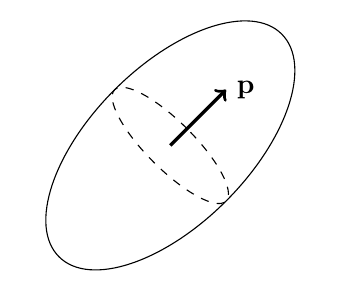
\begin{tikzpicture}[rotate=45]
        \draw(0,0) ellipse (2 cm and 1 cm);
        \draw[dashed](0,0) ellipse (0.3 cm and 1 cm);
        \draw[->,very thick](0,0) --++ (1,0)node[right]{$\textbf{p}$};
    \end{tikzpicture}
    \hfill
    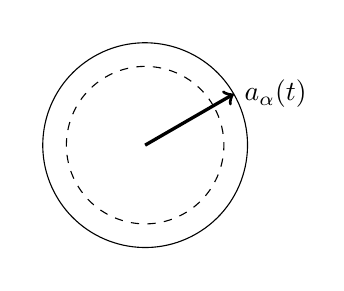
\begin{tikzpicture}[rotate=30]
        \draw(0,0) ellipse (1.3 cm and 1.3 cm);
        \draw[dashed](0,0) ellipse (1 cm and 1 cm);
        \draw[->,very thick](0,0) --++ (1.3,0)node[right]{$a_\alpha(t)$};
    \end{tikzpicture}
    \hfill
    \caption{Scheme of an axis symmetric particle with fore after symmetry and orientation normal vector \textbf{p}.}
    \label{fig:scheme2}
\end{figure}

\subsubsection*{Closures}
Initially we aim to solve the momentum equation for the fluid and particle phase \ref{eq:hybrid_avg_dt_rhou} and \ref{eq:hybrid_avg_dt_dp_alpha}. 
As previously mentioned these equations contain the following closures terms : $\oneavg{\textbf{T}}, \pnnavg{\textbf{f}_\alpha}, \pnnavg{\textbf{t}_\alpha}$ and $\pnnavg{\textbf{S}_\alpha}$ if we discard the fluctuation terms.
The closure for the averaged stress tensor appearing in \ref{eq:hybrid_avg_dt_rhou} can be express assuming solid unreformable motion inside the particles, with, \citep{jackson1997locally},



Notice that the bulk velocity appearing in the above expression is in fact, $\avg{\textbf{u}} = \phi_1\oneavg{u} + \pnavg{\textbf{u}_\alpha} + \div (\pnavg{\mathcal{P}_\alpha})$.
Thus, the moment of momentum appear explicitly in the closure of the stress in agreement with \citet{zhang1997momentum}.  
Regarding the drag force, in  \citet{brenner1963resistance} they demonstrate that in low but finite inertia for an arbitrary shaped particle it could be expressed as,
\begin{equation}
    \textbf{f}_\alpha = 3 \pi \mu L \left[
        \textbf{R}_\alpha \cdot \textbf{U}
        + \frac{3}{16} Re  \left(
            3 \textbf{R}_\alpha 
            - \textbf{I} (\textbf{R}_\alpha : \textbf{e} \textbf{e})
        \right)
        \textbf{R}_\alpha\cdot  \textbf{U}
    \right]
\end{equation}
\JL{je pense pas que ce soit utile de citer Brenner \& Cox. On peut se limiter au regime de Stokes et juste dire que $\textbf{R}_\alpha$ depend de $\textbf{pp}$}
where $\textbf{U} = \oneavg{\textbf{u}}(\textbf{x}_\alpha)  - \textbf{u}_\alpha$ , $\textbf{e} = \textbf{U}/|\textbf{U}|$. 
and,  $\textbf{R}_\alpha$ is the resistance tensor in the laboratory frame. 
Besides, for axisymmetric particles with orientation vector \textbf{p} (sse \ref{fig:scheme2}) it can be shown that $\textbf{R}_\alpha = (R_{||} - R_\bot) \textbf{pp} + R_\bot \textbf{I}$, where $R_{||}$, $R_\bot$ are scalar coefficients \citep{guazzelli2011,kim2013microhydrodynamics}. 
Regarding the hydrodynamic torque applied on an asymmetric particle it can be expressed in Stokes regime as, 
\begin{equation}
    \textbf{t}_\alpha 
    = 
    \textbf{R}_{\omega T}\cdot \mathbf{\Omega}
     + \textbf{R}_{TU} \cdot \textbf{U} 
\end{equation}
where the first term represent the torque acting on the particle due to its translation,
with $R_T$ a correlation also function of the shape and $\textbf{U}$.
It must be noted that this relation remain partially true in low but finite inertial regime. 
Note that the correlation,  $R_T, R_{||} , R_{\bot}$ can be found in \citet{fintzi2023inertial} for cylindrical particles in dilute regime. 
And the second term represent the torque due to its rotation vector $\omega_\alpha$, where $\textbf{R}_{\omega T}$ is the resistance tensor linking rotation and torque \citet{pierson2021hydrodynamic} for inertial regime.  
Both $\textbf{R}_{\omega T}$ and $\textbf{R}_{TU}$ terms are function of the orientation of the particle \textbf{p}.
Closure for $\textbf{S}_\alpha$ can also be found but in the stokes regime only, 
indeed theoretical results are given in \citet[p 62]{kim2013microhydrodynamics}. Nevertheless, we do not provide them here as the expression is rather complicated. 
From the view of these closure terms we can see that in addition to the zeroth order terms, it is primordial to determine quantitatively the tensor $\textbf{pp}$, the rate of rotation $\omega_\alpha$ and the moment of momentum $\mathcal{P}_\alpha$. 

\subsubsection*{Dipole equations}
\JL{pourquoi dipole equations et pas first order moment equations ? l'expression dipole est utilise en mecanique des fluides mais pour des ecoulements potentiels generalement.}
Let consider a solid axis symmetric particle with fore after symmetric such that exposed in \ref{fig:scheme2}. 
Due to axis symmetric nature of the particle we can stipulate that, 
\begin{equation}
    \mathcal{M}_\alpha =  \textbf{pp} (M_\alpha^{||} - M_\alpha^\bot) 
    +  \textbf{I} M_\alpha^\bot
    \label{eq:M_definition}
\end{equation}
with $M_\alpha^{||}$, $M_\alpha^\bot$ being constant values related to the volume and shape of the particle. 
Besides, the velocity fields in inside each particle's domain can be deduced from solid body assumption, $\textbf{u}_2(\textbf{x}_\alpha + \textbf{r},t) = \textbf{u}_\alpha + \omega_\alpha \times \textbf{r}$ where $\omega_\alpha$ is the rotation vector of the particle $\alpha$.
By making use of this velocity decomposition it is easy to show that,
\begin{align}
    \mathcal{P}_\alpha
    &=  \omega_\alpha \times \left[
        \textbf{pp}(M_\alpha^{||} - M_\alpha^\bot) 
        + \textbf{I} M_\alpha^\bot
    \right]
    \label{eq:P_edfinition}\\
    2\mathcal{S}_\alpha
    &=  (M_\alpha^{||} - M_\alpha^\bot) \left(
        \omega_\alpha \times
        \textbf{pp}
        + \textbf{pp} \times \omega_\alpha
    \right)
    \label{eq:S_definition}\\
    \mu_\alpha / 
    &= \omega_\alpha \cdot \left[
        \textbf{pp} 
    (M_\alpha^{||}  - M_\alpha^{\bot} ) 
    - \textbf{I}(M_\alpha^{||} + M_\alpha^{\bot})
    \right]
    = \omega_\alpha \cdot\mathcal{I}_\alpha
    \label{eq:mu_definition}
\end{align}
Remark that  using the definition of $\mathcal{I}_\alpha$ yields a much simpler expression for $\mu_\alpha$. 

It is then straightforward to show that from \ref{eq:hybrid_avg_dt_dM_alpha},\ref{eq:S_definition} and \ref{eq:M_definition} we obtain the second order moment of volume conservation,
\begin{equation}
    \pddt (\pnavg{\textbf{pp}})
    + \div (
        \pnavg{\textbf{pp}\textbf{u}_\alpha}
        )
    = 
    \pnavg{\textbf{pp} \times \omega_\alpha}
    + \pnavg{\omega_\alpha \times \textbf{pp}} 
    % + \pnavg{\textbf{pp}' \times \omega_\alpha'}
    % +\pnavg{\omega_\alpha' \times \textbf{pp}'}
    \label{eq:hybrid_avg_dt_pp}
\end{equation}
In stokes flow we can find closure in the hypothesis of torque free particle, see \citet{kim2013microhydrodynamics}
\begin{equation}
    \omega_\alpha \times \textbf{p} 
    = -  \textbf{p} \times \omega_\alpha 
    = \avg{\Omega} \cdot \textbf{p} + \xi(\avg{\textbf{E}} \cdot \textbf{p} - \avg{\textbf{E}} \cdot \textbf{ppp})
    \label{eq:stokes_closure}
\end{equation}
Here $\avg{\textbf{E}}$ and $\avg{\Omega}$ are the symmetric and antisymmetric part of the velocity gradient. 
Injecting \ref{eq:stokes_closure} into \ref{eq:hybrid_avg_dt_pp} directly gives,
\begin{multline}
    \pddt (\pnavg{\textbf{pp}})
    + \div (
        \pnavg{\textbf{pp}\textbf{u}_\alpha}
        )
    = 
    \avg{\Omega} \cdot \pnavg{\textbf{pp}} 
    - \pnavg{\textbf{pp}} \cdot \avg{\Omega} \\
    + \beta\left[
        \avg{\textbf{E}} \cdot \pnavg{\textbf{pp}} 
        -\pnavg{\textbf{pp}} \cdot \avg{\textbf{E}} 
    - \avg{\textbf{E}} : \avg{\textbf{pppp}}
    \right]
    % \label{eq:hybrid_avg_dt_pp}
\end{multline}

In agreement with \citet{advani1987use} which found similar results except that they brought empirical expression for the fluctuation terms. \JL{je ne vois pas bien ou tu trouves cette equation dans le papier de Advani et Tucker ? D'ailleurs as tu lu Wang et Tucker 2008. Il est a mon avis plus explicite sur ce genre de chose.}

An equation for the rotation rate $\pnnavg{\omega_\alpha}$ can be obtained by, manipulating the angular momentum balance  \ref{eq:hybrid_avg_dt_dmu_alpha}, and using \ref{eq:mu_definition} and \ref{eq:hybrid_avg_dt_pp}, which gives,
\begin{multline}
    \left(
        \pnnavg{\textbf{pp}} 
        - \textbf{I}\frac{M_\alpha^{||} + M_\alpha^\bot}{M_\alpha^{||} - M_\alpha^\bot}
    \right)\left[
        \pddt (\pnavg{\omega_\alpha})
        + \div (
            \pnavg{\omega_\alpha}\pnnavg{\textbf{u}_\alpha}
            + \pnavg{\omega_\alpha'\textbf{u}_\alpha'})
        \right]\\
    +  \pnavg{\omega_\alpha}
    \cdot(\pnnavg{\omega_\alpha} 
    \times \pnnavg{\textbf{pp}})
    = \frac{\pnavg{\textbf{t}_\alpha}}{\rho_2}
    -\pnavg{\omega_\alpha' \cdot (\omega_\alpha \times \textbf{pp})'}
    +\pnavg{\omega_\alpha' \times \textbf{pp}}
    - \pnavg{\textbf{pp}'\dot{ \omega_\alpha}'}
\end{multline}
On the RHS we can observe that there is numerous closure fluctuation terms.  
\tb{FIND ref of this equations}\JL{as tu compare cette equation a celle de Zhang et Prosperreti 1997 ? }
\tb{they make spherical particle only so it is not interesting }
\subsubsection*{Stress equation}

Lastly, once we solved for $\pnnavg{\textbf{pp}}$ and $\pnavg{\omega_\alpha}$ we can deduce $\mathcal{S}_\alpha$ thanks to \ref{eq:S_definition}.
Afterward, we compute the integral of the undefined internal stress with \ref{eq:hybrid_avg_dt_dS_alpha}, which yield in our case, 
\begin{multline}
    \pnavg{\int_{\Omega_\alpha} 
        \mathbf{T}_2
    d\Omega}
    =  
      \pnavg{\textbf{S}_\alpha}
    - \rho_2\pnavg{\ddt \mathcal{S}_\alpha}\\
    - (M_\alpha^{||} - M_\alpha^\bot) \pnavg{
        (\omega_\alpha \times \textbf{p}) (\omega_\alpha \times \textbf{p}) } 
    -M_\alpha^\bot \pnavg{\textbf{I} \omega_\alpha^2 -\omega_\alpha\omega_\alpha }
    \label{eq:T2_definition}
\end{multline}
Then considering the particle nature it is possible to deduce its mean deformation from the stress integral, and validate or not the irreformability hypothesis made at start. 
It is also possible to compute the trace of the stress using \ref{eq:hybrid_avg_dt_dD_alpha}, yielding in this case, 
\begin{equation}
    \pnnavg{\int_{\Omega_\alpha} 
        \textbf{I}:\mathbf{T}_2
    d\Omega}
    =  
     (M_\alpha^{||} + M_\alpha^\bot) \pnnavg{
    \omega_\alpha^2} 
    - (M_\alpha^{||} - M_\alpha^\bot) \pnnavg{
    \omega_\alpha\omega_\alpha :  \textbf{pp}}
    + \pnnavg{\textbf{M}_\alpha} : \textbf{I}
\end{equation}
where we considered that the volume of the particle remained constant. 
This equation means that the rotational acceleration contribute to the isotropic particle pressure. 


In a pure rigorous manner the equivalent bulk stress of the suspension yield, 
\begin{equation*}
    \avg{\textbf{T}} = 
    \phi_1 \oneavg{\textbf{T}} 
    + \pnavg{\int_{\Omega_\alpha} \mathbf{T}_2 d\Omega}
    -\div \pnavg{\int_{\Omega_\alpha} \textbf{r}\mathbf{T}_2 d\Omega}
    + \ldots
\end{equation*}
Where the first and second terms on the RHS are given by \ref{eq:T_definition} and \ref{eq:T2_definition}, and the last one can be obtained with the third order moment of momentum equations. 
Anyhow, if we neglect this last term and if the solid motion hypothesis remain true we can determine the bulk stress using \ref{eq:T2_definition} which gives,
\begin{multline*}
    \avg{\textbf{T}} = 
    - \phi_1\oneavg{p}\textbf{I} 
    + \mu_1 \avg{\textbf{E}} 
    + \frac{1}{2}\frac{\pnavg{\textbf{S}_\alpha}}{\rho_2}
    - (M_\alpha^{||} - M_\alpha^\bot) \pnavg{\ddt \left(
        \omega_\alpha \times
        \textbf{pp}
        + \textbf{pp} \times \omega_\alpha
    \right)}\\
    - (M_\alpha^{||} - M_\alpha^\bot) \pnavg{
        (\omega_\alpha \times \textbf{p}) (\omega_\alpha \times \textbf{p}) } 
    -M_\alpha^\bot \pnavg{\textbf{I} \omega_\alpha^2 -\omega_\alpha\omega_\alpha }
\end{multline*}
\todo[inline]{Include an order and show the self torque part}
Each term on the RHS can be for one part factorized by \textbf{I} yieldings the equivalent pressure of the suspension, and an other part by $\avg{\textbf{E}}$ yielding the equivalent viscosity. 



\tb{
\subsubsection*{Oblate bubbles}

As it has already mentioned the trace of the moment of momentum equation can be used to derive the Reyl
It is also possible to derive from the second moment of mass equation an equation for the mean aspect ratio $\pnnavg{\xi}$ of the particles.
Indeed, let's consider obalte particles, such as droplets or bubble, in this case the second moment of mass can be written, $\mathcal{M}_\alpha =  \textbf{pp} [M_\alpha^{||}(t) - M_\alpha^\bot(t)] +  \textbf{I} M_\alpha^\bot(t)$
\tb{As in tomiyama example they state that the shape of the particle is of particular importance here the moment of volume matter }


\subsubsection*{Spherical compressible bubbles}
As mentioned in the \ref{sec:Lagrangian} from teh trace of the moment of momentum equation we can recover the Rayleigh-Lamb-Plesset equation.
Thus, by using the averaged moment of momentum equation we can falll back on \citet{zhang1994ensemble} model.

\subsubsection*{Slightly deformable elastic particle}

Now let consider the momentum conservation of slightly deformable particles.
First, the velocity field inside the particles, is assumed linear and incompressible, such that $\textbf{u}(\textbf{y}_\alpha) = \textbf{u}_\alpha + \mathcal{L}_\alpha \cdot \textbf{r}$ where the second order tensor  $\mathcal{L}_\alpha= \textbf{e}_\alpha+ \boldsymbol{\omega}$, with $\textbf{e}$ and $\boldsymbol{\omega}$ are symmetric and skew-symmetric tensors, respectively.
It directly follows from the expression of the velocity : $\mathcal{P}_\alpha = \int_{\Omega_\alpha} \textbf{r}\textbf{u} d\Omega = \mathcal{L}_\alpha\cdot \mathcal{M}$

The constitutive equation of the stress, $\textbf{T}_2$, within the particle phase can be written such as $\textbf{T}_2 = \mathbb{C} : \textbf{e}_2$ for elastic materials, with $\mathbb{C}$ the fourth order stiffness tensor and $ \textbf{e}_2 = \frac{1}{2}\left(\grad\textbf{u}_2+(\grad\textbf{u}_2)^T\right)$ is the rate of strain symmetric tensor.
Making use of the internal velocity expression yield directly the relation, $\textbf{e}_2=\textbf{e}_\alpha\cdot$ in $\Omega_\alpha$.

We know that the deformation of the particles will not have an explicit impact on the linear conservation equations.
Thus, we will be interested into the first and second order momentum and mass conservation equations respectively.
Making use of the average of \ref{eq:dt_P_alpha} over every configuration of the flow, and using the previous properties yield an equation for the average stress tensor within the suspension, namely,
\begin{equation}
    \pnnavg{\int_{\Omega_\alpha}\textbf{T}_\alpha d\Omega}
    = n_p\mathbb{C} : \pnnavg{(\mathcal{L}_\alpha+ \mathcal{L}_\alpha^T) v_\alpha}
    % = - \mathcal{L}_\alpha\cdot \mathcal{L}_\alpha\cdot \mathcal{M}_\alpha
    % - \mathcal{M}_\alpha \cdot\ddt \mathcal{L}_\alpha
    % - \textbf{M}_\alpha
    \label{eq:hybrid_avg_dt_P_alpha}
\end{equation}
\begin{equation}
    \mathcal{M}_\alpha \cdot\ddt \mathcal{L}_\alpha
    = - \mathcal{L}_\alpha\cdot \mathcal{L}_\alpha\cdot \mathcal{M}_\alpha
    - \mathbb{C} : (\mathcal{L}_\alpha+ \mathcal{L}_\alpha^T) v_\alpha
    - \textbf{M}_\alpha
    \label{eq:hybrid_avg_dt_P_alpha}
\end{equation}
Besed on that kind of argument \citet{lhuillier1987phenomenology}
}


One last remark is in order. 
With \ref{eq:dt_S_alpha} it is possible to compute the integral of the undefined internal stress $\int_{\Omega_\alpha} 
\mathbf{T}_2
d\Omega$ within the particle phase.
But first,  for a prolate spheroid the $\textbf{S}_\alpha$ may be written with this quite lenthly expression : 
\begin{multline}
    \textbf{S}_\alpha 
    = \frac{20}{3}\pi \mu a^3 \left[
    \left(
        X^M \mathbf{p}^{(0)}+Y^M \mathbf{p}^{(1)}+Z^M \mathbf{p}^{(2)}
    \right) : \textbf{E}\right.\\ \left.
    + \frac{3}{5} Y^H ((\mathbf{\Omega} - \omega_\alpha) \times \textbf{pp} + \textbf{pp} \times (\mathbf{\Omega} - \omega_\alpha) )
    \right]
    \label{eq:S_def}
\end{multline}
where, $X^M$, $Y^M$,  $Z^M$ and $Y^H$ are scalar resistance function related to the shape of the particles, and the $\mathbf{p}^{(i)}$ are fourth order orientation tensor solely express in terms of $\textbf{p}$, all of which are given in \citet[p 62.]{kim2013microhydrodynamics}. 
theerfore, by rearranging the term for the integrated stress, \ref{eq:dt_S_alpha}, can be written for axissymmetric particles such as, 
\begin{multline}
    \pnavg{\int_{\Omega_\alpha} 
        \mathbf{T}_2
    d\Omega}
    =  
      \pnavg{\textbf{S}_\alpha}
    - (M_\alpha^{||} - M_\alpha^\bot)\pnavg{\ddt  \left(
        \omega_\alpha \times
        \textbf{pp}
        + \textbf{pp} \times \omega_\alpha
    \right) }\\
    - (M_\alpha^{||} - M_\alpha^\bot) \pnavg{
        (\omega_\alpha \times \textbf{p}) (\omega_\alpha \times \textbf{p}) } 
    -M_\alpha^\bot \pnavg{\textbf{I} \omega_\alpha^2 -\omega_\alpha\omega_\alpha }
\end{multline}
which is a constitutive expression of the stress. 
In stokes flow condition one may argue that all product of $\omega_\alpha$ and time derivative of $\omega$ are negligible, leavening with the stresslet. 